% Training, likelihood, generation and decoding for next-token predictors,
% shared by the NNDS CNN deck and the NN transformer deck. Moved from
% Lecture_CNNs.tex by Claude (2026-11-16).

\begin{frame}{Training a next-token predictor}
    \setlength{\parskip}{3pt}
    \setlength{\abovedisplayskip}{4pt}
    \setlength{\belowdisplayskip}{4pt}

    We train on a \myalert{shifted target}: the input is $z_0,\ldots,z_{T-1}$
    and the target is the same text moved by one position, $z_1,\ldots,z_T$.
    Each prediction $\vc{p}_t$ is compared with the next ID, averaging the
    cross-entropy over the $T$ input positions:
    \[
        \mathcal{L}=-\frac{1}{T}\sum_{t=0}^{T-1}
        \log\idx{\vc{p}_t}{z_{t+1}}.
    \]

    During training we feed the true tokens (\myalert{teacher forcing}), \NNDSorNN{so a
    causal CNN computes all predictions in parallel without seeing future targets.}{as
    in the open-loop setting of the recurrent lectures. The model must be causal,
    so that $\vc{p}_t$ never sees its own target $z_{t+1}$.}

\end{frame}

\begin{frame}{A probabilistic view}
    \setlength{\parskip}{4pt}
    \setlength{\abovedisplayskip}{6pt}
    \setlength{\belowdisplayskip}{6pt}

    Consider the probability $p(\vc{z})$ of a whole sequence. By the \NNDSorNN{product
    rule of probability}{chain rule of probability, as for time series in the
    recurrent lectures}, we can always write it as
    \[
        p(\vc{z})=\prod_{t=0}^{T-1}p(z_{t+1}\mid z_0,\ldots,z_t),
    \]
    where $z_0$ is a fixed start token, so it needs no factor. A causal model estimates every factor
    with the same network, $p(z_{t+1}\mid z_0,\ldots,z_t)\approx\idx{\vc{p}_t}{z_{t+1}}$.

    Our loss is then $\mathcal{L}=-\frac{1}{T}\log p(\vc{z})$: training
    maximizes the likelihood of the training texts. A model of $p(\vc{z})$
    over text is a \myalert{language model}. Since we can sample new sequences
    from it, it is also a \myalert{generative model}.

    \SlideSource{Section 8.4 of \NNDSorNN{the book}{\textit{Alice's Adventures in a Differentiable Wonderland}}.}

\end{frame}

\begin{frame}{Autoregressive models}
    \setlength{\parskip}{4pt}
    \setlength{\abovedisplayskip}{6pt}
    \setlength{\belowdisplayskip}{6pt}

    The same next-token predictor can generate text in an
    \myalert{autoregressive} way\NNDSorNN{}{, as in the free-running forecasts
    of the recurrent lectures}.

    We prompt it with the beginning of the sequence and sample the next token
    from the predicted distribution. We concatenate its ID to the input and
    call the model again, continuing one token at a time. For example:
    \[
        \texttt{Check}
        \quad\longrightarrow\quad
        \texttt{Check this}
        \quad\longrightarrow\quad
        \texttt{Check this out}\quad\ldots
    \]

    The input now includes the model's own sampled tokens. As in the linear
    models lecture, we can sample with a \myalert{temperature} $\tau$: a small
    $\tau$ gives predictable text, a large $\tau$ more varied text.

    \NNDSorNN{Training can compute many next-token predictions in parallel.}{During
    training, all the input tokens are known in advance.} Generation
    must wait for each sampled token before predicting the following one.

\end{frame}

\begin{whiteframe}{Autoregressive generation}
    \setlength{\abovecaptionskip}{5pt}
    \setlength{\parskip}{4pt}

    \begin{figure}
        \centering
        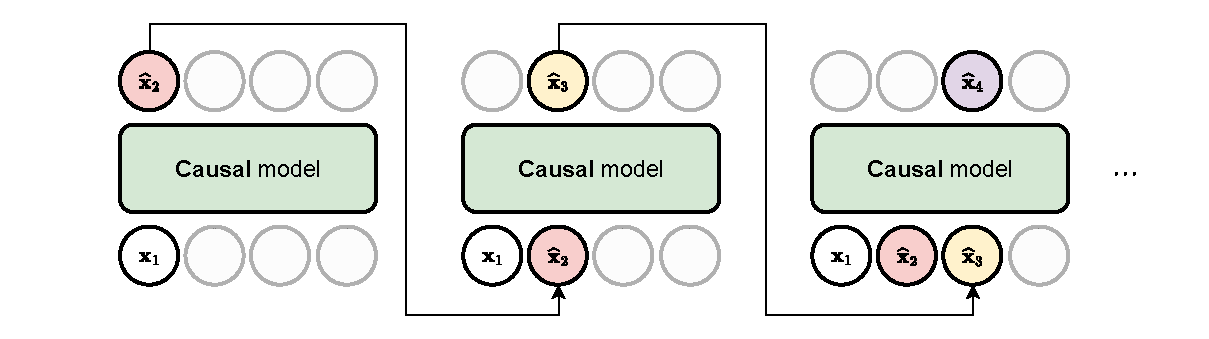
\includegraphics[width=0.95\textwidth,height=0.42\textheight,keepaspectratio]{images/text/autoregressive_generation.pdf}
        \caption{The hat marks a generated value: $\hat{x}_{t+1}$ is the model's prediction
            for position $t+1$, which is fed back as the next input. For text, we feed back
            sampled token IDs. Gray circles mark unused positions.}
    \end{figure}

\end{whiteframe}

\begin{frame}{Decoding strategies}
    \setlength{\parskip}{4pt}

    The rule we use to pick each token from $\vc{p}_t$ is called
    \myalert{decoding}:
    \begin{itemize}
        \item \textbf{Greedy decoding} always takes the most probable token.
              Since $p(\vc{z})$ is a product of many factors, a likely token now
              can lead to an unlikely sequence later.
        \item \textbf{Sampling} draws the token from $\vc{p}_t$, with a
              temperature $\tau$ ($\tau\to0$ recovers greedy). Top-$k$ and
              top-$p$ sampling first discard the unlikely tail.
        \item \textbf{Beam search} keeps the $k$ partial sequences with the
              highest $\log p$, extends each of them, and keeps the best $k$
              again.
    \end{itemize}

    \SlideSource{Holtzman et al. (2020), \href{https://arxiv.org/abs/1904.09751}{\textit{The Curious Case of Neural Text Degeneration}}, ICLR.}

\end{frame}

% Figure: shared/assets/images/text/decoding_tree.tex (Claude, 2026-11-05).
\begin{whiteframe}{Greedy decoding and beam search}

    \begin{center}
        % Editable figure: two decoding steps after the prompt "the". Edge labels are
% next-token probabilities; the column on the right is p of each sequence.
% Greedy decoding (orange) and beam search with k=2 (green) end differently.
% Written by Claude (2026-11-05).
\begingroup
\begin{tikzpicture}[x=1cm,y=1cm,
        tok/.style={draw=drawgray,fill=drawgray_l,rounded corners=1.5pt,line width=0.6pt,
            minimum height=0.48cm,inner sep=2.5pt,font=\small\ttfamily},
        edge/.style={line width=0.8pt,draw=drawgray!60},
        greedy/.style={line width=1.6pt,draw=draworange},
        beam/.style={line width=1.6pt,draw=drawgreen},
        prob/.style={font=\footnotesize,fill=white,inner sep=1pt},
        seq/.style={font=\small,anchor=west}]
    \node[tok] (r) at (0,0) {the};
    \node[tok] (a) at (2.6,0.9) {cat};
    \node[tok] (b) at (2.6,-0.9) {dog};
    \node[tok,anchor=west] (aa) at (4.9,1.35) {sat};
    \node[tok,anchor=west] (ab) at (4.9,0.45) {is};
    \node[tok,anchor=west] (ba) at (4.9,-0.45) {barks};
    \node[tok,anchor=west] (bb) at (4.9,-1.35) {runs};
    \draw[greedy] (r.east) -- node[prob] {0.5} (a.west);
    \draw[beam] (r.east) -- node[prob] {0.4} (b.west);
    \draw[greedy] (a.east) -- node[prob] {0.4} (aa.west);
    \draw[edge] (a.east) -- node[prob] {0.3} (ab.west);
    \draw[beam] (b.east) -- node[prob] {0.9} (ba.west);
    \draw[edge] (b.east) -- node[prob] {0.1} (bb.west);
    \node[font=\small\bfseries] at (7.5,1.85) {$p(\text{sequence})$};
    \node[seq,text=draworange] at (6.8,1.35) {$0.20$ \enspace greedy};
    \node[seq,text=drawgray] at (6.8,0.45) {$0.15$};
    \node[seq,text=drawgreen!70!black] at (6.8,-0.45) {$0.36$ \enspace beam, $k=2$};
    \node[seq,text=drawgray] at (6.8,-1.35) {$0.04$};
\end{tikzpicture}
\endgroup

    \end{center}

    \vspace{0.6em}
    Keeping \texttt{dog} lets beam search find a more likely sequence.

\end{whiteframe}
